\chapter{Background}\label{C:related}

This chapter explores the current research conducted in this area. It then covers the key ideas needed to understand the remainder of the report. These ideas are -- approaches to storing method coverage, edit distance metrics, evaluating performance of Java programs and the use of grid computing.

\section{Related Work}
\label{relatedworkRef}
\subsection{Identifying Redundant Tests}
Testing is a critical part to any software engineering process, not only to stop incidents stemming from the product, but also partially related to the increase in popularity of agile methodologies \cite{chaos}. Many of these methodologies use test driven development and continuous integration. This results in testing becoming more important throughout the development process. For these reasons there have been research papers that examine the different approaches taken to identify redundant test cases and reduce the size of test suites \cite{wong1995effect, wong1999test, rothermel1998empirical, rothermel2002empirical,koochakzadeh2009test,zhang2011empirical,li2008static}.

Whether programmatically reducing a test suite's size is worth the trade off in the ability to locate bugs is unclear.  Wong et al. \cite{wong1995effect, wong1999test} explored the impact that reducing the size of the test suite based off of code coverage had on the fault detection capability. By introducing faults into several programs and comparing the performance between the original and reduced test suites, they found that test suite reduction did not severely impact fault detection capability. In contrast to this finding, Rothermel et al. \cite{rothermel1998empirical, rothermel2002empirical} further expanded on Wong's work by using different benchmark's and performance metrics. They found that test-suite reduction can severely impact the fault detection capability. The conflicting studies create uncertainty. This motivates our research to decouple the removal of tests from the tool and move the responsibility onto developers. 

A popular technique used in detecting redundancy involves analysing the statement executions, known as statement coverage. Maurer, Garousi and Koochakzadeh \cite{koochakzadeh2009test} attempt to answer the question, \textit{is coverage information enough to determine redundant test cases?} They state a redundant test case as being one that does not improve a specific criteria. For example, Figure \ref{fig:venndiagram} represents the statement criteria data from test cases T1 to T5. The figure shows that T4 and T5 are fully redundant as T3 covers the statements executed by these tests. The authors looked at two other criteria, branch coverage and granularities. Granularity criteria involved splitting the tests into setup, exercise (execution), verify (assert) and lastly teardown then performing analysis over each section. They implemented two different metrics in which both used the criteria described above. The first metric examined each individual test with every other test. It was calculated by measuring the percentage of a test case that is also a subset of another test case. The second metric examined each test case with the test suite as a whole. It was calculated by measuring the percentage of the test case that the test suite covered without the test in it. By comparing with manual inspection, they were able to determine the level of false positive and actual redundant tests. Of the redundant tests manually identified, the algorithm matched 95\% of those. However, of the tests that were manually identified as being non-redundant, 52\% of these were identified as being redundant by the algorithm. They concluded that coverage-based information is vulnerable in giving false-positives when identifying redundant test cases, suggesting common code paths as being a root cause. Statement coverage criteria gave a high rate of detection, but the implementation allowed for false positives to impact the results. 

\begin{figure}[h]
\begin{center}
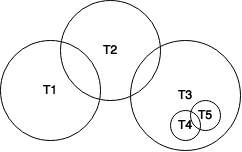
\includegraphics[width=10cm, height=6cm]{VennDiagram.png}
\end{center}
\caption{The coverage of each test is shown by a circle. It shows that T4 and T5 are redundant as T3 already covers those statements.}
\label{fig:venndiagram}
\end{figure}

Zhang, Marinov, Zhang and Khurshid \cite{zhang2011empirical} examined the use of a greedy technique in comparison to heuristics.This required a criteria to be set by the tester, for example, statement coverage. The greedy technique would greedily select a test case that satisfies the maximum number of unsatisfied test requirements. It would continue until all the test requirements had been satisfied. The new test suite will contain exactly the same coverage as the old test suite while removing redundant test cases. This means that if a test subsumed another, then it would always be removed. The heuristic implementation was first conceived by Harrold, Gupta and Soffa \cite{harrold1993methodology} where it selects essential test cases as early as possible. Essential being that only one test case satisfies a test requirement exclusively. The heuristic approach resulted in the most cost-effective reduction, this being the amount of reduction and the fault-detection capability of the reduced test suites. This showed that although greedy approach worked, there were better techniques available.

In situations where it is not possible to generate a spectrum to analyse, static analysis can be used to determine the level of redundancy. Robinson, Li and Francis \cite{li2008static} explore this. The tests for the benchmark they use are written in a high level automation framework and consist of a list of commands. The commands perform actions such as file copying and loading configurations. To identify redundant test cases they examine the test case commands as well as the instructions within the procedures that the test case loads. To calculate the similarities between two test cases, they consider three different metrics. These are the Manhattan distance, unigram cosine similarity and bigram cosine similarity. They each were measuring how closely related two tests were based on the sequence of commands and procedures loaded. Their findings were similar to Maurer et al. \cite{koochakzadeh2009test} in that there are a large number of false positives. Static checking has several limitations in comparison to dynamic. The main disadvantage is the availability of data. During run-time is when a large portion of the data trail is available. This is important when needing to know the exact method calls and parameters passed to these methods. Static checking would provide useful information in a framework where dynamic data can not be collected. The framework would also need to be applicable to being examined in a static fashion such as the one used by Robinson, Li and Francis \cite{li2008static}.

Taking into the related work discussed, each paper used the coverage of a test suite at several different criterion levels but none looked at the method execution explicitly. This leaves a potentially useful approach to the problem that may help determine the level of redundancy within a test suite. 
\subsection{Calling Tree}
When methods execute there is a trail of data that is left behind. Piecing together this data can show the relationships between methods, which is known as a \textit{call graph}. The call graph can be retrieved statically or dynamically \cite{graham1982gprof}. A static graph represents every possible run of the program. A dynamic graph represents one particular run. Comparing them, a static graph requires more information to be held. In the particular case of profiling test cases, dynamic would be more suitable due to the nature of a test case being the same for every run. Another advantage of a dynamic graph is the ability to collect functional parameters. Xiaotong Zhuang and et al. \cite{Zhuang06accurate} describe a call tree as the overall tree of every method execution. To store the full call tree would involve an excess of memory, therefore they discuss the use of a calling context tree. This tree represents the same method executions however is compressed where the edge between the nodes contains a weighting, the weighting being the number of occurrences of that method execution (calling frequency). Examining Figure \ref{fig:callgraph} shows the different variations that can be observed with the same data. The top left hand picture shows the method execution trail, where A calls B, then B calls D twice and A calls C, then C calls D once. The call graph image (top right) condenses the information into one node per method call. This method is the most condensed variation, but gives the least amount of information. Directly below this, the calling context tree condenses it slightly less. It separates each path into its own branch when it is unique to the tree. The connection between nodes contains a weighting which represents the frequency. Finally, the bottom left (call tree) creates a new path for every new method execution regardless of the uniqueness. This allows for the tree to retain the most information about the context.

\begin{figure}[h]
\begin{center}
\includegraphics[width = \textwidth]{CallGraph.png}
\end{center}
\caption{A diagram showing the three different variations of Call Graph information. Where  each have a varying level of information that is stored.}
\label{fig:callgraph}
\end{figure}

\subsection{Edit Distance Metrics}
\label{editdistbg}
Edit distance algorithms play an important part in many domains, ranging from signal processing to mutations in genome sequences \cite{navarro2001guided}. They calculate the number of edit operations needed to go from one string to another, in our research they are used to calculate the difference between test spectrums. There are a variety of different implementations of edit distance metrics. Cohen, Ravikumar and Fienberg \cite{cohen2003comparison} explore different edit distance metrics for name matching. They concluded that Monge and Elkan \cite{monge1997efficient} performed the best for string edit-distance metrics. The metric works by splitting the two strings into tokens, the best matching tokens are then calculated to find the similarity using other common metrics such as Levenshtein distance. One of the other techniques they explored was the Levenshtein distance \cite{levenshtein1966binary} metric by itself. This metric is the minimal number of operations to change one test's spectrum into another. These operations are inserting, deleting or substituting and a cost is associated with completing an operation. The maximum difference is the size of the larger spectra. The amount of redundancy is calculated by dividing the cost of operations with the max difference in order to normalize the value. This value is the percentage of the test that is not redundant, the value 1 is then subtracted by the value to give the redundant percentage.

Table \ref{levenTable} shows an example of Levenshtein. The example changes 'kitchen' into 'kitten'. It shows the number of operations needed is 2, and the max potential needed if the two strings were completely different is 7, as kitchen contains 7 characters. The redundancy is calculated by subtracting 1 from the cost over the max potential cost $(1 - (2/7)) $. The outcome being that the words contain 71\% redundant information. 

\begin{table}[H]
\centering

\begin{tabular}{|l|l|l|}
\hline
{\bf Previous State} & {\bf Current State} & {\bf Operation}                      \\ \hline
-                    & kitten              & -                                    \\ \hline
kitten               & kitcen              & Substitution of `t' with `c'         \\ \hline
kitcen               & kitchen             & Insertion of `h' between `c' and `e' \\ \hline
\end{tabular}
\caption{Using Levenshtein edit distance metric to transform kitten to kitchen.}
\label{levenTable}
\end{table}

Table \ref{mongeTable} shows an example of Monge \& Elkan. It compares the strings `paul johnson' and `johson paule'. Each of the strings get broken down into two tokens and the best matches are identified and used for the final score. The table shows that the final score of the Monge \& Elkan is taking into account `paul' \& `paule' and `johnson' \& `johson'. Using these two matches, the final result is 1/2 * (.85 + .80) = 0.825.

\begin{table}[H]
\centering

\begin{tabular}{|l|l|}
\hline
\textbf{Input string 1:}        & paul johnson \\ \hline
\textbf{Input string 2:}        & johson paule \\ \hline
                                &              \\ \hline
Levenshtein("paul","johson")    & 0.00         \\ \hline
Levenshtein("paul","paule")     & 0.80         \\ \hline
Levenshtein("johnson","paule")  & 0.00         \\ \hline
Levenshtein("johnson","johson") & 0.85         \\ \hline
\end{tabular}
\caption{The Monge \& Elkan edit distance metric to calculate the similarity between "paul johnson" and "johson paule"}
\label{mongeTable}
\end{table}



\subsection{Wilcoxon Signed Rank Test}

A Wilcoxon Signed Rank test is used to infer whether there are any significant differences between the techniques implemented in this report. The Wilcoxon Signed Rank test was first proposed by Frank Wilcoxon in 1945 \cite{wilcoxon1945individual}. It is a nonparametric test for comparing two pair groups. A nonparametric test is a collective term that is given to inferences that are valid under less confining assumptions than classical statistical inferences \cite{nonparametric}. The test does not assume that the data follows a normal distribution which is ideal for the data presented in our research and is used when two nominal variables and one measure variable is being measured \cite{mcdonald2009handbook}.

\section{Performance Evaluation}
\label{performanceEvalBG}
Throughout the report different techniques are designed and implemented to identify redundant test cases. To evaluate the techniques, experiments are conducted and must adhere to a standard procedure. The purpose for evaluating the performance of a given technique is to create an understanding of the typical performance. For this typical performance to be valid, it has to be rigorous in design and implementation. This involves taking into consideration a variety of factors that will be examined in reference to research papers that explore the issues.

Andy Georges et al. \cite{georges2007statistically} and Steve Blackburn et al. \cite{blackburn2008wake} present issues and alternatives to the current Java performance methodologies used in research papers. They note that in premier conferences, 16 of the 50 papers examined did not discuss the methodology they used. This limits the validity of the results and creates a situation where the experiment cannot be reproduced. One of the main issues identified is specifying singular numbers, without expressing what the number is referring to (average, median, best, worst). This leads to a misleading representation of the results. A set of parameters that are of interest are explored in the paper, these include, heap size, start up performance, number of virtual machine (VM) invocations and handling of garbage collection. An experiment should also take into consideration the environment that the analysis is executed on:
\begin{itemize}
\item \textbf{Heap Size} -- A change in heap size can impact the garbage collection process. The smaller the heap size, the more often the garbage collector is run.
\item \textbf{Start Up Costs}  -- The costs associated with starting the application up. This will always involve class loading and just in time (JIT) re(compilation), it can also involve reading from a database and setting the application up.
\item \textbf{Number of VM invocations} -- The number of application runs that a single VM instance will execute.
\item \textbf{Garbage Collection} -- The process in identifying and removing objects that are no longer referenced.
\item \textbf{Environment} -- The hardware that the application is being run on.
\end{itemize}

\section{Grid Computing}
The time intensive nature of conducting the experiments resulted in a single computer not being adequate. A grid computing system was used instead, it is a distributed system of multiple machines that have no interactive tasks between each other. No interactions results in task independence being a necessity. The particular grid system used for this report is located at Victoria University of Wellington. The machines in the grid are idle machines around the School of Engineering and Computer Science. There are a limited number of machines, therefore a total of 150 jobs can be run at a given time. Since the grid is located around an active community, if a user logs on while a process is being conducted, the application is paused until the machine returns to an idle state.